\subsection{Ροή πληροφορίας} \label{subsection:4-3-9-data-flow}

Στην παρούσα υποενότητα θα αναλυθεί η ροή της πληροφορίας στο σύστημα. Λόγω των πολλαπλών υπηρεσιών, της κατάτμησης την πληροφορίας και των διαφορετικών σημείων αποθήκευσης της, η ροή της πληροφορίας στο σύστημα ακολουθεί ένα σχετικά περίπλοκο μονοπάτι (σε σχέση με κλασσικές, μονολιθικές, κεντροποιημένες εφαρμογές).

Αρχικά θα γίνει αναφορά στη διαδικασία αποθήκευσης των νέων πληροφοριών. Η μοναδική πηγή παραγωγής δεδομένων στο σύστημα είναι οι χρήστες και κατ' επέκταση η υπηρεσία Concordia Application, εφόσον είναι η μοναδική υπηρεσία με την οποία αυτοί αλληλεπιδρούν. Τα δεδομένα που δημιουργούν οι χρήστες (πληροφορίες χρηστών, τίτλοι θεμάτων και περιεχόμενο μηνυμάτων) κατατέμνονται πριν αποθηκευτούν. Η πληροφορία που εισάγεται στο σύστημα διαχωρίζεται σε δύο μέρη. Στο blockchain αποθηκεύεται ένας δείκτης προς τα δεδομένα, ενώ τα πραγματικά δεδομένα αποθηκεύονται στη βάση OrbitDB. Ο δείκτης εκτός από την άμεση χρησιμότητα στην εύρεση των δεδομένων, παρέχει και την έμμεση λειτουργικότητα της δημιουργίας απαραίτητων μεταδομένων όπως ο αριθμός των θεμάτων στο σύστημα ή των μηνυμάτων σε ένα θέμα.

Από την πλευρά της εύρεση των πληροφοριών στο σύστημα, η ροή είναι ως εξής. Αρχικά, είναι απαραίτητη η αναζήτηση στο blockchain για την εύρεση του δείκτη προς τα δεδομένα. Έπειτα, τα δεδομένα μπορούν να ανακτηθούν μέσω του IPFS από τον εκάστοτε χρήστη ή από κάποιον Pinner.

Τέλος, παρακάτω δίνεται ένα παράδειγμα εισαγωγής πληροφορίας στο σύστημα και έπειτα ανάκτησης της ίδιας πληροφορίας.

Έστω, χρήστης που δημιουργεί νέο θέμα. Τα δεδομένα που παράγονται είναι ο τίτλος του θέματος και το περιεχόμενο του πρώτου μηνύματος. Μεταδεδομένα της δημιουργίας είναι η διεύθυνση του/της δημιουργού του θέματος. Για την αποθήκευση του θέματος στο σύστημα δημιουργείται πρώτα συναλλαγή στο blockchain ώστε να δημιουργηθεί μία νέα εγγραφή στον πίνακα των θεμάτων. Η εγγραφή αυτή δεν περιέχει τίποτα παρά μόνο τη διεύθυνση του/της δημιουργού χρήστη. Αν η συναλλαγή είναι επιτυχής, θα επιστραφεί ο αύξων αριθμός του νέου θέματος. Έπειτα, στην προσωπική βάση OrbitDB του/της χρήστη και στον πίνακα των θεμάτων θα προστεθεί εγγραφή με αναγνωριστικό τον αύξων αριθμό του θέματος όπου θα αποθηκευτούν τα δεδομένα του τίτλου και πρώτου μηνύματος. Στο σχήμα \ref{figure:4-3-data-flow-insert} παρουσιάζεται γραφικά η διαδικασία.

\begin{figure}[H]
    \centering
    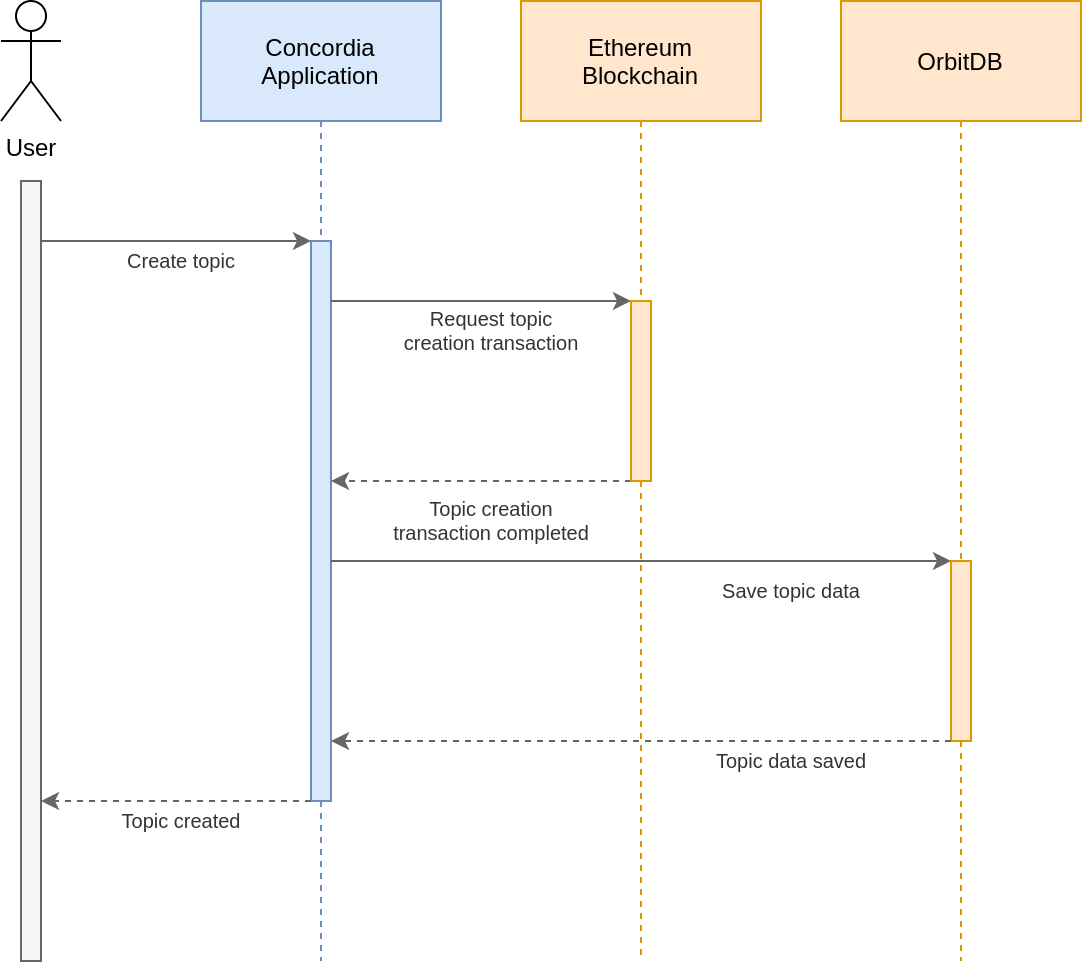
\includegraphics[width=.7\textwidth]{assets/figures/chapter-4/4.3.architecture-4.3.9.data-flow-insert.png}
    \caption{Διάγραμμα ακολουθίας δημιουργίας θέματος}
    \label{figure:4-3-data-flow-insert}
\end{figure}

Έστω, χρήστης που επιθυμεί να διαβάσει το προηγούμενο μήνυμα. Αρχικά, πρέπει να διαβαστεί ο πίνακας θεμάτων από το blockchain. Η πληροφορία αυτή εμπλουτίζεται από τα δεδομένα του κάθε θέματος, τα οποία ανακτώνται από τις προσωπικές βάσεις Orbit κάθε χρήστη. Έπειτα, εφόσον το θέμα βρεθεί και ο αύξων αριθμός του είναι γνωστός, πρέπει να διαβαστούν από το blockchain τα μεταδομένα των μηνυμάτων του θέματος και συγκεκριμένα η διευθύνσεις των δημιουργών τους. Τέλος, μέσω του IPFS πρέπει να γίνει αντιγραφή των προσωπικών βάσεων των δημιουργών του κάθε μηνύματος και να αναζητηθούν σε αυτές τα εκάστοτε μηνύματα. Στο σχήμα \ref{figure:4-3-data-flow-read} φαίνεται το διάγραμμα ροής της πληροφορίας κατά την ανάκτηση πληροφοριών από το σύστημα.

\begin{figure}[H]
    \centering
    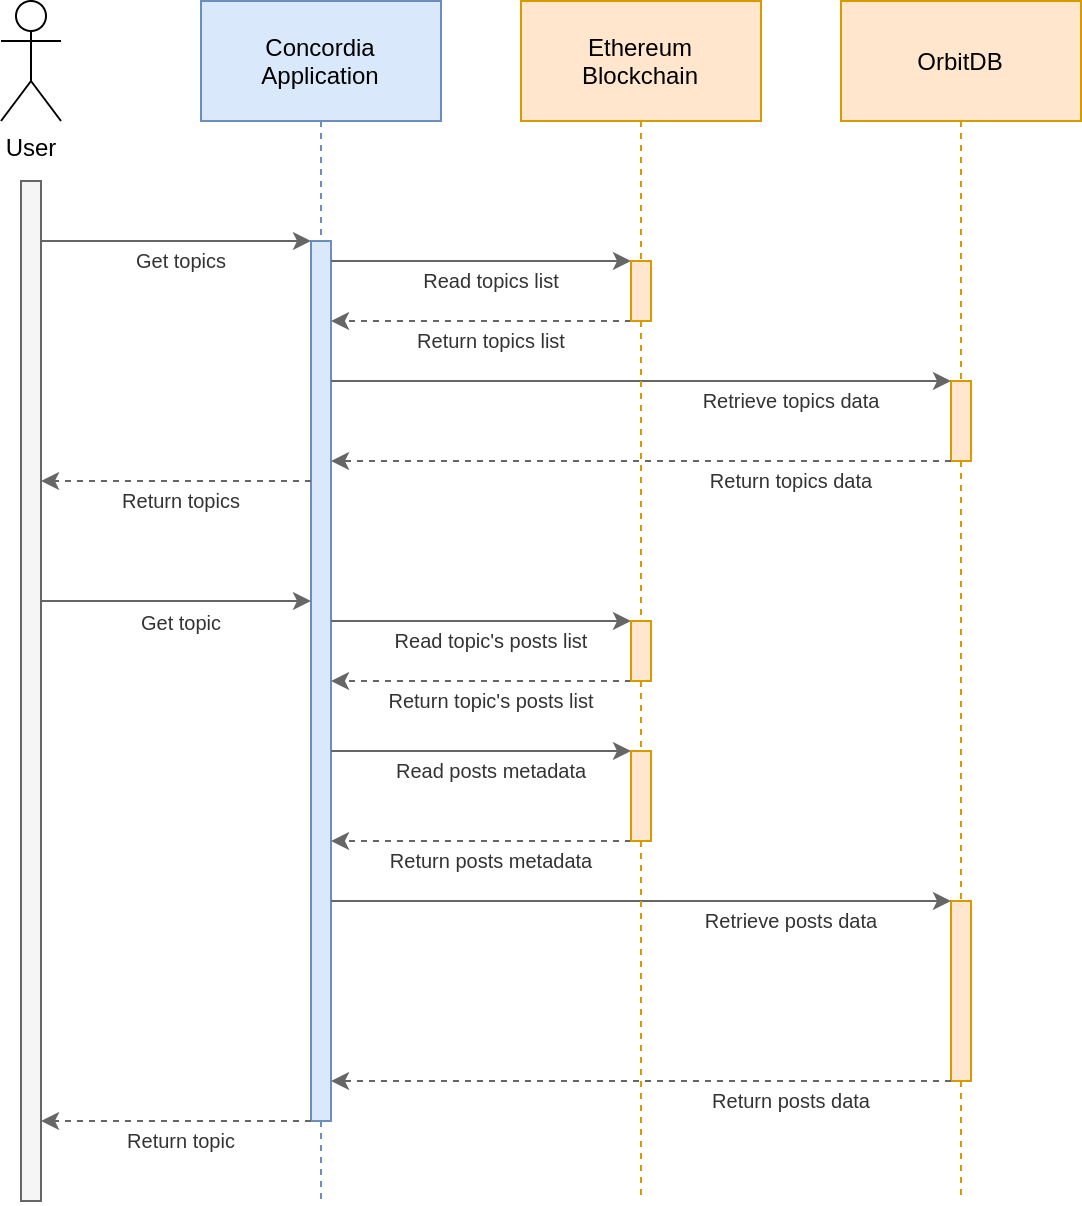
\includegraphics[width=.7\textwidth]{assets/figures/chapter-4/4.3.architecture-4.3.9.data-flow-read.png}
    \caption{Διάγραμμα ακολουθίας εύρεσης και ανάκτησης θέματος}
    \label{figure:4-3-data-flow-read}
\end{figure}